\documentclass{article}

\usepackage{amsmath}
\usepackage{amssymb}
\usepackage{bm}
\usepackage{caption}
\usepackage{color}
\usepackage{CJKutf8}
\usepackage{color}
\usepackage{enumitem}
\usepackage{graphicx}
\usepackage{indentfirst}
\usepackage{listings}
\usepackage{mathdots}
\usepackage{subcaption}
\usepackage{tikz}
\usepackage{wasysym}
\usepackage{xcolor}

\setlength{\parindent}{2em}

\usetikzlibrary{shapes,arrows, automata}

\allowdisplaybreaks

\newcommand{\hytt}[1]{\texttt{\hyphenchar\font=\defaulthyphenchar #1}}
\hyphenation{}

\definecolor{mygreen}{rgb}{0,0.6,0}
\definecolor{mygray}{rgb}{0.5,0.5,0.5}
\definecolor{mymauve}{rgb}{0.58,0,0.82}
%\footnotesize
\lstset{ %
  backgroundcolor=\color{white},   % choose the background color; you must add \usepackage{color} or \usepackage{xcolor}
  basicstyle=\ttfamily,            % the size of the fonts that are used for the code
  breakatwhitespace=false,         % sets if automatic breaks should only happen at whitespace
  breaklines=true,                 % sets automatic line breaking
  captionpos=b,                    % sets the caption-position to bottom
  commentstyle=\ttfamily\color{mygreen},    
                                   % comment style
  deletekeywords={},               % if you want to delete keywords from the given language
  escapeinside={},                 % if you want to add LaTeX within your code
  extendedchars=true,              % lets you use non-ASCII characters; for 8-bits encodings only, does not work with UTF-8
  frame=single,                    % adds a frame around the code
  keepspaces=true,                 % keeps spaces in text, useful for keeping indentation of code (possibly needs columns=flexible)
  keywordstyle=\color{blue},       % keyword style
  language=C++,                    % the language of the code
  morekeywords={},                 % if you want to add more keywords to the set
  numbers=left,                    % where to put the line-numbers; possible values are (none, left, right)
  numbersep=5pt,                   % how far the line-numbers are from the code
  numberstyle=\tiny\color{mygray}, % the style that is used for the line-numbers
  rulecolor=\color{black},         % if not set, the frame-color may be changed on line-breaks within not-black text (e.g. comments (green here))
  showspaces=false,                % show spaces everywhere adding particular underscores; it overrides 'showstringspaces'
  showstringspaces=false,          % underline spaces within strings only
  showtabs=false,                  % show tabs within strings adding particular underscores
  stepnumber=1,                    % the step between two line-numbers. If it's 1, each line will be numbered
  stringstyle=\color{mymauve},     % string literal style
  tabsize=2,                       % sets default tabsize to 2 spaces
  title=\lstname                   % show the filename of files included with \lstinputlisting; also try caption instead of title
}

\begin{document}
\begin{CJK*}{UTF8}{gbsn}
\CJKtilde

\title{表达式语法分析实验报告}

\author{计算机1202 张艺瀚\\学号:20123852}
\maketitle

\section{实验题目}
表达式语法分析

\section{实验目的}
熟悉并设计一个表达式的语法分析器

\section{实验内容}
\begin{enumerate}
\item 设计表达式的语法分析器算法
\item 编写代码并上机调试运行通过
\end{enumerate}

\section{概要设计}

本语法分析器实现了LR(1)和LL(1)语法分析方法,对给定文法自动生成LR(1)和LL(1)分析表,在几个简单文法的测试下正常运行。

下面介绍具体设计实现。

\texttt{SyntaxAnalyzer} 类定义(代码清单~\ref{lst: classdeclarationlst})如下:
\begin{center}
\begin{lstlisting}[caption = {\texttt{SyntaxAnalyzer} 类定义代码清单}, label = {lst: classdeclarationlst}]
class SyntaxAnalyzer
{
public:
	SyntaxAnalyzer(const string& filePath);

	Grammar G;

	void display(const LR0Item& item);
	void display(const LR1Item& item);
	void display(const set<LR0Item>& I);
	void display(const set<LR1Item>& I);
	
	
	vector<set<LR1Item>> lr1ItemSetFamily;
	vector<vector<LR1ActionTabItem>> lr1ActionTab;
	vector<vector<unsigned int>> lr1GoToTab;
	vector<unsigned int> lr1Stack;
	string lr1Input;

	set<LR0Item> LR0Closure(const set<LR0Item>& I);
	set<LR1Item> LR1Closure(const set<LR1Item>& I);
	set<LR1Item> LR1GoTo(const set<LR1Item>& I, char X);
	void calLR1ItemSetFamily();
	void buildLR1ParseTab();
	bool lr1SyntaxAnalyze(const string& myLR1Input);


	vector<vector<LL1Item>> ll1ParseTab;
	vector<char> ll1Stack;
	string ll1Input;

	void buildLL1ParseTab();
	bool ll1SyntaxAnalyze(const string& myLL1Input);

private:

};
\end{lstlisting}
\end{center}

构造函数和~\texttt{display} 多态函数不再赘述,下面分别介绍LR(1)和LL(1)分析器的构造。

\subsection{LR(1)语法分析器的设计实现}
\subsubsection{LR1项的数据结构设计}
代码如下(代码清单~\ref{lst: lr1itemlst})如下:
\begin{center}
\begin{lstlisting}[caption = {LR1项的数据结构设计代码清单}, label = {lst: lr1itemlst}]
class LR1Item
{
public:
	LR1Item() = default;
	LR1Item(const LR0Item& myLR0Item, char myLookaheadSymbol);
	LR1Item(unsigned int myLProductionRuleIdx, unsigned int myRProductionRuleIdx, unsigned int myDotPos, char myLookaheadSymbol);

	unsigned int lProductionRuleIdx;
	unsigned int rProductionRuleIdx;
	unsigned int dotPos;
	char lookaheadSymbol;

	friend bool operator < (const LR1Item& i1, const LR1Item& i2);
	friend bool operator ==(const LR1Item& i1, const LR1Item& i2);
	friend bool operator > (const LR1Item& i1, const LR1Item& i2);
	friend bool operator !=(const LR1Item& i1, const LR1Item& i2);

private:

};

bool operator <(const LR1Item& i1, const LR1Item& i2)
{
	return i1.lProductionRuleIdx < i2.lProductionRuleIdx?
		true: (i1.lProductionRuleIdx > i2.lProductionRuleIdx?
			false: (i1.rProductionRuleIdx < i2.rProductionRuleIdx?
				true: (i1.rProductionRuleIdx > i2.rProductionRuleIdx?
					false: (i1.dotPos < i2.dotPos?
						true: (i1.lookaheadSymbol < i2.lookaheadSymbol)))));
}

bool operator ==(const LR1Item& i1, const LR1Item& i2)
{
	return i1.lProductionRuleIdx == i2.lProductionRuleIdx
		&& i1.rProductionRuleIdx == i2.rProductionRuleIdx
		&& i1.dotPos == i2.dotPos
		&& i1.lookaheadSymbol == i2.lookaheadSymbol;
}

bool operator >(const LR1Item& i1, const LR1Item& i2)
{
	return !(i1 < i2) && !(i1 == i2);
}

bool operator !=(const LR1Item& i1, const LR1Item& i2)
{
	return !(i1 == i2);
}

LR1Item::LR1Item(const LR0Item& myLR0Item, char myLookaheadSymbol):
	lProductionRuleIdx(myLR0Item.lProductionRuleIdx), rProductionRuleIdx(myLR0Item.rProductionRuleIdx), dotPos(myLR0Item.dotPos),
	lookaheadSymbol(myLookaheadSymbol)
{

}

LR1Item::LR1Item(unsigned int myLProductionRuleIdx, unsigned int myRProductionRuleIdx, unsigned int myDotPos, char myLookaheadSymbol):
	lProductionRuleIdx(myLProductionRuleIdx), rProductionRuleIdx(myRProductionRuleIdx), dotPos(myDotPos), lookaheadSymbol(myLookaheadSymbol)
{

}
\end{lstlisting}
\end{center}

\subsubsection{\texttt{LR1Closure} 成员函数的设计实现}
\texttt{LR1Closure} 类定义(代码清单~\ref{lst: lr1closurelst})如下:
\begin{center}
\begin{lstlisting}[caption = {\texttt{LR1Closure} 成员函数代码清单}, label = {lst: lr1closurelst}]
set<LR1Item> SyntaxAnalyzer::LR1Closure(const set<LR1Item>& I)
{
	set<LR1Item> ret;
	for(auto ptr = I.begin(); ptr != I.end(); ++ptr)
	{
		ret.insert(*ptr);
	}

	bool updated = true;
	while(updated)
	{
		updated = false;

		for(auto ptr = ret.begin(); ptr != ret.end(); ++ptr)
		{
			if(ptr->dotPos < G.P[ptr->lProductionRuleIdx].rPartSet[ptr->rProductionRuleIdx].size()
				&& G.isNonTerminal(G.P[ptr->lProductionRuleIdx].rPartSet[ptr->rProductionRuleIdx][ptr->dotPos]))
			{
				ProductionRule pr;
				int prIdx = G.getProductionRuleByLeft(pr, G.P[ptr->lProductionRuleIdx].rPartSet[ptr->rProductionRuleIdx][ptr->dotPos]);
				for(size_t i = 0; i < pr.rPartSet.size(); ++i)
				{
					string str;
					if(ptr->dotPos + 1 < G.P[ptr->lProductionRuleIdx].rPartSet[ptr->rProductionRuleIdx].size())
					{
						str = G.P[ptr->lProductionRuleIdx].rPartSet[ptr->rProductionRuleIdx][ptr->dotPos + 1] + ch2str(ptr->lookaheadSymbol);
					}
					else
					{
						str = ch2str(ptr->lookaheadSymbol);
					}
					set<char> s = G.getFirst(str);
					int oldSize = ret.size();
					for(auto& sPtr: s)
					{
						if(sPtr != 'e')
						{
							ret.insert(LR1Item(prIdx, i, 0, sPtr));
						}
					}
					int newSize = ret.size();
					if(oldSize != newSize)
					{
						updated = true;
					}
				}
			}
		}
	}

	// cout << "LR1Closure:\n"; display(ret); cout << endl;

	return ret;
}
\end{lstlisting}
\end{center}

\subsubsection{\texttt{LR1GoTo} 成员函数的设计实现}
代码(代码清单~\ref{lst: lr1gototablst})如下:
\begin{center}
\begin{lstlisting}[caption = {\texttt{LR1GoTo} 成员函数代码清单}, label = {lst: lr1gototablst}]
set<LR1Item> SyntaxAnalyzer::LR1GoTo(const set<LR1Item>& I, char X)
{
	if(find(G.VN.begin(), G.VT.begin(), X) != G.VN.end()
		|| find(G.VT.begin(), G.VT.end(), X) != G.VT.end())
	{
		set<LR1Item> ret;

		for(auto ptr = I.begin(); ptr != I.end(); ++ptr)
		{
			if(ptr->dotPos < G.P[ptr->lProductionRuleIdx].rPartSet[ptr->rProductionRuleIdx].size()
				&& G.P[ptr->lProductionRuleIdx].rPartSet[ptr->rProductionRuleIdx][ptr->dotPos] == X)
			{
				ret.insert(LR1Item(ptr->lProductionRuleIdx, ptr->rProductionRuleIdx, ptr->dotPos + 1, ptr->lookaheadSymbol));
			}
		}

		// cout << "LR1GoTo:\n"; display(LR1Closure(ret)); cout << endl;
		
		return LR1Closure(ret);
	}
	else
	{
		return set<LR1Item>();
	}
}
\end{lstlisting}
\end{center}

\subsubsection{\texttt{calLR1ItemSetFamily} 成员函数的设计实现}
代码(代码清单~\ref{lst: callr1itemsetfamilylst})如下:
\begin{center}
\begin{lstlisting}[caption = {\texttt{calLR1ItemSetFamily}代码清单}, label = {lst: callr1itemsetfamilylst}]
void SyntaxAnalyzer::calLR1ItemSetFamily()
{
	G.P.push_back(ProductionRule('S', vector<string>({ch2str(G.S)})));
	sort(G.P.begin(), G.P.end(),
		[](const ProductionRule& pr1, const ProductionRule& pr2)
		{
			return pr1.lPart < pr2.lPart?
				true: (pr1.lPart > pr2.lPart?
					false: pr1.rPartSet[0] < pr2.rPartSet[0]);
		});

	G.VN.push_back('S');
	sort(G.VN.begin(), G.VN.end());

	G.S = 'S';

	G.nullable.clear();
	G.first.clear();
	G.follow.clear();
	G.nullable.assign(G.VN.size(), false);
	G.first.assign(G.VN.size() + G.VT.size(), set<char>());
	G.follow.assign(G.VN.size(), set<char>());

	G.display();

	G.calNullableFirstFollow();

	lr1ItemSetFamily.push_back(
		LR1Closure(
			set<LR1Item>({
				LR1Item(
					find_if(
						G.P.begin(), G.P.end(),
						[](const ProductionRule& pr)
						{
							return pr.lPart == 'S';
						}) - G.P.begin(),
					0, 0, '$'
					)
				})
			)
		);

	bool updated = true;
	while(updated)
	{
		updated = false;

		for(auto& itemSetPtr: lr1ItemSetFamily)
		{
			for(auto& symbolPtr: G.VN)
			{
				set<LR1Item> itemSet = LR1GoTo(itemSetPtr, symbolPtr);
				if(!itemSet.empty()
					&& find_if(lr1ItemSetFamily.begin(), lr1ItemSetFamily.end(),
						[itemSet](const set<LR1Item>& s)
						{
							if(s.size() != itemSet.size())
							{
								return false;
							}
							else
							{
								auto ptr1 = itemSet.begin();
								auto ptr2 = s.begin();
								for(; ptr1 != itemSet.end(); ++ptr1, ++ptr2)
								{
									if(!(*ptr1 == *ptr2))
									{
										return false;
									}
								}
								return true;
							}
						}) == lr1ItemSetFamily.end())
				{
					lr1ItemSetFamily.push_back(itemSet);
					updated = true;
				}
			}

			for(auto& symbolPtr: G.VT)
			{
				set<LR1Item> itemSet = LR1GoTo(itemSetPtr, symbolPtr);
				if(!itemSet.empty()
					&& find_if(lr1ItemSetFamily.begin(), lr1ItemSetFamily.end(),
						[itemSet](const set<LR1Item>& s)
						{
							if(s.size() != itemSet.size())
							{
								return false;
							}
							else
							{
								auto ptr1 = itemSet.begin();
								auto ptr2 = s.begin();
								for(; ptr1 != itemSet.end(); ++ptr1, ++ptr2)
								{
									if(!(*ptr1 == *ptr2))
									{
										return false;
									}
								}
								return true;
							}
						}) == lr1ItemSetFamily.end())
				{
					lr1ItemSetFamily.push_back(itemSet);
					updated = true;
				}
			}
		}
	}

	// sort lr1ItemSetFamily
	sort(lr1ItemSetFamily.begin(), lr1ItemSetFamily.end(),
		[](const set<LR1Item>& itemSet1, const set<LR1Item>& itemSet2)
		{
			auto ptr1 = itemSet1.begin();
			auto ptr2 = itemSet2.begin();
			for(; ptr1 != itemSet1.end() && ptr2 != itemSet2.end(); ++ptr1, ++ptr2)
			{
				if(*ptr1 > *ptr2)
				{
					return false;
				}
				else if(*ptr1 < *ptr2)
				{
					return true;
				}
			}
			if(ptr1 != itemSet1.end() && ptr2 == itemSet2.end())
			{
				return false;
			}
			else
			{
				return true;
			}
		});

	cout << "item set family" << endl;
	for(size_t i = 0; i < lr1ItemSetFamily.size(); ++i)
	{
		cout << "I" << i << endl;
		display(lr1ItemSetFamily[i]);
		cout << endl;
	}

	cout << "Goto graph" << endl;
	for(size_t i = 0; i < lr1ItemSetFamily.size(); ++i)
	{
		for(size_t j = 0; j < G.VT.size(); ++j)
		{
			set<LR1Item> Ij = LR1GoTo(lr1ItemSetFamily[i], G.VT[j]);
			if(!Ij.empty())
			{
				cout << "I" << i << endl;
				display(lr1ItemSetFamily[i]);
				cout << "receives " << G.VT[j] << ", goes to" << endl;
				display(Ij);
				cout << endl;
			}
		}

		for(size_t j = 0; j < G.VN.size(); ++j)
		{
			set<LR1Item> Ij = LR1GoTo(lr1ItemSetFamily[i], G.VN[j]);
			if(!Ij.empty())
			{
				cout << "I" << i << endl;
				display(lr1ItemSetFamily[i]);
				cout << "receives " << G.VN[j] << ", goes to" << endl;
				display(Ij);
				cout << endl;
			}
		}
	}
}
\end{lstlisting}
\end{center}

我们使用增广文法,即添加产生式$S' \rightarrow S$。这时,文法的终结符集,开始符,\texttt{nullable} 集,\texttt{first} 集和~\texttt{follow} 集均需重新计算。这些计算仅与文法相关,文法及其上操作的设计实现见~\ref{sec: appendix} 附录。

\subsubsection{\texttt{buildLR1ParseTab} 成员函数的设计实现}
代码(代码清单~\ref{lst: buildlr1parsetablst})如下:
\begin{center}
\begin{lstlisting}[caption = {\texttt{buildLR1ParseTab} 成员函数代码清单}, label = {lst: buildlr1parsetablst}]
void SyntaxAnalyzer::buildLR1ParseTab()
// notice that the lookahead symbol may be e!!!
{
	lr1ActionTab.assign(lr1ItemSetFamily.size(), vector<LR1ActionTabItem>(G.VT.size() + 1, LR1ActionTabItem(ERR, 0, 0, 0)));
	lr1GoToTab.assign(lr1ItemSetFamily.size(), vector<unsigned int>(G.VN.size(), lr1ItemSetFamily.size()));
	// if an item in lr1GoToTab equals to the value of lr1ItemSetFamily.size(), it means this item is invalid

	for(size_t i = 0; i < lr1ItemSetFamily.size(); ++i)
	{
		for(auto itemSetPtr = lr1ItemSetFamily[i].begin(); itemSetPtr != lr1ItemSetFamily[i].end(); ++itemSetPtr)
		{
			auto VTPtr = find(G.VT.begin(), G.VT.end(), itemSetPtr->lookaheadSymbol);
			auto VNPtr = find(G.VN.begin(), G.VN.end(), itemSetPtr->lookaheadSymbol);
			if(itemSetPtr->dotPos < G.P[itemSetPtr->lProductionRuleIdx].rPartSet[itemSetPtr->rProductionRuleIdx].size())
			{
				if(G.P[itemSetPtr->lProductionRuleIdx].rPartSet[itemSetPtr->rProductionRuleIdx] == "e")
				{
					lr1ActionTab[i][(VTPtr == G.VT.end())? G.VT.size(): (VTPtr - G.VT.begin())] =
						LR1ActionTabItem(REDUCE, itemSetPtr->lProductionRuleIdx, itemSetPtr->rProductionRuleIdx, 0);
				}

				auto ptr = find(G.VT.begin(), G.VT.end(),
					G.P[itemSetPtr->lProductionRuleIdx].rPartSet[itemSetPtr->rProductionRuleIdx][itemSetPtr->dotPos]);
				if(ptr != G.VT.end())
				{
					set<LR1Item> Ij = LR1GoTo(lr1ItemSetFamily[i],
						G.P[itemSetPtr->lProductionRuleIdx].rPartSet[itemSetPtr->rProductionRuleIdx][itemSetPtr->dotPos]);
					int lr1ActionTabCol = ptr - G.VT.begin();
					lr1ActionTab[i][lr1ActionTabCol] = LR1ActionTabItem(
						SHIFT, 0, 0,
						find_if(lr1ItemSetFamily.begin(), lr1ItemSetFamily.end(),
							[Ij](const set<LR1Item>& s)
							{
								if(s.size() != Ij.size())
								{
									return false;
								}
								else
								{
									auto ptr1 = Ij.begin();
									auto ptr2 = s.begin();
									for(; ptr1 != Ij.end(); ++ptr1, ++ptr2)
									{
										if(!(*ptr1 == *ptr2))
										{
											return false;
										}
									}
									return true;
								}
							}) - lr1ItemSetFamily.begin()
						);
				}
			}
			else
			{
				if(G.P[itemSetPtr->lProductionRuleIdx].lPart != 'S')
				{
					int lr1ActionTabCol = (VTPtr == G.VT.end())? G.VT.size(): (VTPtr - G.VT.begin());
					lr1ActionTab[i][lr1ActionTabCol] = LR1ActionTabItem(REDUCE, itemSetPtr->lProductionRuleIdx, itemSetPtr->rProductionRuleIdx, 0);
				}
				else
				{
					lr1ActionTab[i][G.VT.size()] = LR1ActionTabItem(ACCEPT, 0, 0, 0);
				}
			}
		}
	}

	for(size_t i = 0; i < lr1ItemSetFamily.size(); ++i)
	{
		for(size_t A = 0; A < G.VN.size(); ++A)
		{
			set<LR1Item> Ij = LR1GoTo(lr1ItemSetFamily[i], G.VN[A]);
			lr1GoToTab[i][A] = find_if(lr1ItemSetFamily.begin(), lr1ItemSetFamily.end(),
				[Ij](const set<LR1Item>& s)
				{
					if(s.size() != Ij.size())
					{
						return false;
					}
					else
					{
						auto ptr1 = Ij.begin();
						auto ptr2 = s.begin();
						for(; ptr1 != Ij.end(); ++ptr1, ++ptr2)
						{
							if(!(*ptr1 == *ptr2))
							{
								return false;
							}
						}
						return true;
					}
				}) - lr1ItemSetFamily.begin();
		}
	}

	cout << "lr1ActionTab" << endl;
	for(size_t i = 0; i < lr1ActionTab.size(); ++i)
	{
		for(size_t j = 0; j < lr1ActionTab[i].size(); ++j)
		{
			cout << "lr1ActionTab[" << i << "," << ((j == G.VT.size())? '$': G.VT[j]) << "] = ";
			switch(lr1ActionTab[i][j].action)
			{
				case SHIFT: cout << "SHIFT " << lr1ActionTab[i][j].itemSetIdx << endl; break;
				case REDUCE: cout << "REDUCE "; G.P[lr1ActionTab[i][j].lProductionRuleIdx].display(); cout << endl; break;
				case ACCEPT: cout << "ACCEPT" << endl; break;
				default: cout << "ERR" << endl;
			}
		}
	}
	cout << endl;

	cout << "lr1GoToTab" << endl;
	for(size_t i = 0; i < lr1GoToTab.size(); ++i)
	{
		for(size_t j = 0; j < lr1GoToTab[i].size(); ++j)
		{
			cout << "lr1GoToTab[" << i << "," << G.VN[j] << "] = "
			     << ((lr1GoToTab[i][j] == lr1ItemSetFamily.size())? " ": to_string(lr1GoToTab[i][j])) << endl;
		}
	}
}
\end{lstlisting}
\end{center}

\subsubsection{\texttt{lr1SyntaxAnalyze} 成员函数的设计实现}
代码(代码清单~\ref{lst: lr1syntaxanalyzelst})如下:
\begin{center}
\begin{lstlisting}[caption = {\texttt{lr1SyntaxAnalyze} 成员函数代码清单}, label = {lst: lr1syntaxanalyzelst}]
bool SyntaxAnalyzer::lr1SyntaxAnalyze(const string& myLR1Input)
{
	if(myLR1Input.size() == 0)
	{
		cout << "Input is empty!" << endl;
		return false;
	}

	cout << "Parsing " << myLR1Input << "..." << endl;

	lr1Stack.push_back(
		find_if(
			lr1ItemSetFamily.begin(), lr1ItemSetFamily.end(),
			[this](const set<LR1Item>& s)
			{
				return find_if(s.begin(), s.end(),
					[this](const LR1Item& i)
					{
						return G.P[i.lProductionRuleIdx].lPart == 'S';
					}) != s.end();
			}
			) - lr1ItemSetFamily.begin()
		);

	string str = myLR1Input;
	reverse(str.begin(), str.end());
	lr1Input = "$" + str;

	int idx = lr1Input.size() - 1;
	char a = lr1Input[idx];
	for(;;)
	{
		unsigned int s = lr1Stack[lr1Stack.size() - 1];
		auto ptr = find(G.VT.begin(), G.VT.end(), a);
		int aIdx = (ptr == G.VT.end())? G.VT.size(): ptr - G.VT.begin();
		LR1ActionTabItem curAction = lr1ActionTab[s][aIdx];
		cout << "Begin a new pass..." << endl;
		cout << "Current state(top of the stack): "
		     << lr1Stack[lr1Stack.size() - 1] << endl;
		display(lr1ItemSetFamily[lr1Stack[lr1Stack.size() - 1]]);
		cout << "Current input symbol: " << a << endl << endl;
		if(curAction.action == SHIFT)
		{
			lr1Stack.push_back(curAction.itemSetIdx);
			cout << "Push back state " << curAction.itemSetIdx << endl;
			display(lr1ItemSetFamily[curAction.itemSetIdx]);
			--idx;
			a = lr1Input[idx];
			cout << "Shift and now the input symbol is " << a << endl << endl;
		}
		else if(curAction.action == REDUCE)
		{
			cout << "Reduce using production rule "
			     << G.P[curAction.lProductionRuleIdx].lPart << "->"
			     << G.P[curAction.lProductionRuleIdx].rPartSet[curAction.rProductionRuleIdx] << endl;
			int num = (G.P[curAction.lProductionRuleIdx].rPartSet[curAction.rProductionRuleIdx] == "e")?
				0: G.P[curAction.lProductionRuleIdx].rPartSet[curAction.rProductionRuleIdx].size();
			for(int i = 0; i < num; ++i)
			{
				lr1Stack.erase(lr1Stack.end() - 1);
			}
			cout << "Pop " << num << " state(s) out of the stack" << endl;
			cout << "Now the stack top is state " << lr1Stack[lr1Stack.size() - 1] << endl;
			display(lr1ItemSetFamily[lr1Stack[lr1Stack.size() - 1]]);
			int t = lr1Stack[lr1Stack.size() - 1];
			lr1Stack.push_back(lr1GoToTab[t][find(G.VN.begin(), G.VN.end(), G.P[curAction.lProductionRuleIdx].lPart) - G.VN.begin()]);
			cout << "lr1GoToTab[" << t << "," << G.P[curAction.lProductionRuleIdx].lPart << "] = "
			     << ((lr1GoToTab[t][find(G.VN.begin(), G.VN.end(), G.P[curAction.lProductionRuleIdx].lPart) - G.VN.begin()] == lr1ItemSetFamily.size())?
			        	" ": to_string(lr1GoToTab[t][find(G.VN.begin(), G.VN.end(), G.P[curAction.lProductionRuleIdx].lPart) - G.VN.begin()]));
			cout << ", so we push back state "
			     << lr1GoToTab[t][find(G.VN.begin(), G.VN.end(), G.P[curAction.lProductionRuleIdx].lPart) - G.VN.begin()] << endl;
			display(lr1ItemSetFamily[lr1GoToTab[t][find(G.VN.begin(), G.VN.end(), G.P[curAction.lProductionRuleIdx].lPart) - G.VN.begin()]]);
			cout << endl;
		}
		else if(curAction.action == ACCEPT)
		{
			cout << "Parsing succeed!" << endl << endl;
			return true;
		}
		else
		{
			cout << "Parsing error!" << endl;
			cout << "In state " << lr1Stack[lr1Stack.size() - 1] << endl;
			display(lr1ItemSetFamily[lr1Stack[lr1Stack.size() - 1]]); cout << endl;
			return false;
		}
	}
}
\end{lstlisting}
\end{center}

我们使用\text{\$}作为分析栈初始栈顶符号。
	
\section{LL(1)语法分析器的设计实现}
\subsubsection{\texttt{buildLL1ParseTab} 成员函数的设计实现}
代码(代码清单~\ref{lst: buildll1parsetablst})如下:
\begin{center}
\begin{lstlisting}[caption = {\texttt{buildLL1ParseTab} 成员函数代码清单}, label = {lst: buildll1parsetablst}]
void SyntaxAnalyzer::buildLL1ParseTab()
{
	ll1ParseTab.assign(G.VN.size(), vector<LL1Item>(G.VT.size() + 1, LL1Item(G.P.size(), 0)));

	for(size_t i = 0; i < G.P.size(); ++i)
	{
		unsigned int AIdx = find(G.VN.begin(), G.VN.end(), G.P[i].lPart) - G.VN.begin();

		for(size_t j = 0; j < G.P[i].rPartSet.size(); ++j)
		{
			set<char> firstAlpha = G.getFirst(G.P[i].rPartSet[j]);

			for(auto& p: firstAlpha)
			{
				unsigned int aIdx = find(G.VT.begin(), G.VT.end(), p) - G.VT.begin();
				if(aIdx < G.VT.size())
				{
					ll1ParseTab[AIdx][aIdx] = LL1Item(i, j);					
				}
			}

			if(find(firstAlpha.begin(), firstAlpha.end(), 'e') != firstAlpha.end())
			{
				set<char> followA = G.getFollow(G.P[i].lPart);
				
				for(auto& p: followA)
				{
					unsigned int bIdx = find(G.VT.begin(), G.VT.end(), p) - G.VT.begin();
					ll1ParseTab[AIdx][bIdx] = LL1Item(i, j);
				}

				if(find(followA.begin(), followA.end(), '$') != followA.end())
				{
					ll1ParseTab[AIdx][G.VT.size()] = LL1Item(i, j);
				}
			}
		}
	}

	for(size_t i = 0; i < ll1ParseTab.size(); ++i)
	{
		for(size_t j = 0; j < ll1ParseTab[i].size(); ++j)
		{
			cout << "ll1ParseTab[" << G.VN[i] << ", " << ((j == G.VT.size())? '$': G.VT[j]) << "] = ";
			if(ll1ParseTab[i][j].i < G.P.size())
			{
				cout << G.P[ll1ParseTab[i][j].i].lPart << "->" << G.P[ll1ParseTab[i][j].i].rPartSet[ll1ParseTab[i][j].j];
			}
			cout << endl;
		}
	}
}
\end{lstlisting}
\end{center}

\subsubsection{\texttt{ll1SyntaxAnalyze} 成员函数的设计实现}
代码(代码清单~\ref{lst: ll1syntaxanalyzelst})如下:
\begin{center}
\begin{lstlisting}[caption = {\texttt{ll1SyntaxAnalyze} 成员函数代码清单}, label = {lst: ll1syntaxanalyzelst}]
bool SyntaxAnalyzer::ll1SyntaxAnalyze(const string& myLL1Input)
{
	if(myLL1Input.size() == 0)
	{
		cout << "Input is empty!" << endl;
		return false;
	}

	cout << "Parsing " << myLL1Input << "..." << endl;

	string str = myLL1Input;
	reverse(str.begin(), str.end());
	ll1Input = '$' + str;
	ll1Stack.push_back('$');
	ll1Stack.push_back(G.S);
	int ip = ll1Input.size() - 1;
	char x = ll1Stack[ll1Stack.size() - 1];

	while(x != '$')
	{
		if(x == ll1Input[ip])
		{
			ll1Stack.erase(ll1Stack.end() - 1);
			--ip;
		}
		else if(find(G.VT.begin(), G.VT.end(), x) != G.VT.end())
		{
			cout << "Parsing error!" << endl;
			return false;
		}
		else
		{
			unsigned int row = find(G.VN.begin(), G.VN.end(), x) - G.VN.begin();
			unsigned int col = (ll1Input[ip] == '$')? G.VT.size(): (find(G.VT.begin(), G.VT.end(), ll1Input[ip]) - G.VT.begin());

			if(ll1ParseTab[row][col].i >= G.P.size())
			{
				cout << "Parsing error!" << endl;
				return false;
			}
			else
			{
				cout << G.P[ll1ParseTab[row][col].i].lPart << "->" << G.P[ll1ParseTab[row][col].i].rPartSet[ll1ParseTab[row][col].j] << endl;
				ll1Stack.erase(ll1Stack.end() - 1);
				if(!(G.P[ll1ParseTab[row][col].i].rPartSet[ll1ParseTab[row][col].j].size() == 1 &&
					G.P[ll1ParseTab[row][col].i].rPartSet[ll1ParseTab[row][col].j][0] == 'e'))
				{				
					for(int cnt = G.P[ll1ParseTab[row][col].i].rPartSet[ll1ParseTab[row][col].j].size() - 1; cnt >= 0; --cnt)
					{
						ll1Stack.push_back(G.P[ll1ParseTab[row][col].i].rPartSet[ll1ParseTab[row][col].j][cnt]);
					}
				}
			}
		}
		x = ll1Stack[ll1Stack.size() - 1];
	}

	cout << "Parsing succeed!" << endl;
	return true;
}
\end{lstlisting}
\end{center}

我们使用\text{\$}作为分析栈初始栈顶符号。

\section{测试数据及运行结果}
该语法分析器对下面的3个测试语法正确运行。

文法~\ref{eq: grammar1}:
\begin{equation}
\begin{aligned} \label{eq: grammar1}
E &\rightarrow TA \\
A &\rightarrow +TA|-TA|\varepsilon \\
T &\rightarrow FB \\
B &\rightarrow *FB|/FB|\varepsilon \\
F &\rightarrow (E)|0|1|2|3|4|5|6|7|8|9 \\
\end{aligned}
\end{equation}

文法~\ref{eq: grammar2}:
\begin{equation} \label{eq: grammar2}
\begin{aligned}
E &\rightarrow E+T|E-T|T \\
T &\rightarrow T*F|T/F|F \\
F &\rightarrow (E)|0|1|2|3|4|5|6|7|8|9 \\
\end{aligned}
\end{equation}

文法~\ref{eq: grammar3}:
\begin{equation} \label{eq: grammar3}
\begin{aligned}
Z &\rightarrow AA \\
A &\rightarrow aA|b \\
\end{aligned}
\end{equation}

对于文法~\ref{eq: grammar3} 和含左递归的文法~\ref{eq: grammar2},LR(1)语法分析器可正确生成分析表,对于不含左递归的文法~\ref{eq: grammar1},LL(1)语法分析器可正确生成分析表。利用自动生成的分析表,LR(1)和LL(1)语法分析器均可正确解析下面的书写正确的复杂的一位数含括号四则运算表达式:
\[ \texttt{1+(1-3*(2-(8+9-7*6/2)/3+9+(1+3)-2)+1)/4} \]
均不能正确解析书写错误的表达式(最后一个4之前缺少一个运算符):
\[ \texttt{1+(1-3*(2-(8+9-7*6/2)/3+9+(1+3)-2)+1)4} \]

运行结果截图如下:

\begin{figure}
\centering
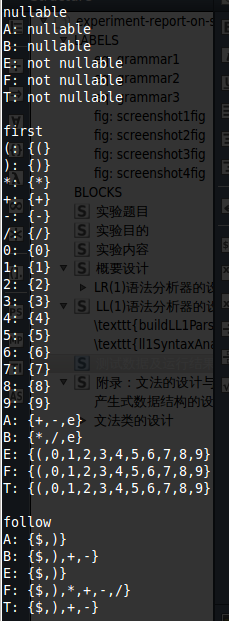
\includegraphics[width=0.5\textwidth]{grammar.png}
\caption{文法}
\label{fig: grammarfig}
\end{figure}

\begin{figure}
        \centering
        \begin{subfigure}[b]{0.3\textwidth}
                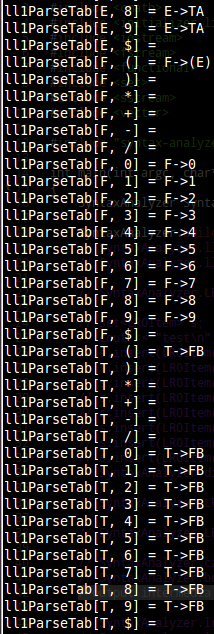
\includegraphics[width=\textwidth]{ll1.png}
                \caption{LL(1)分析表}
                \label{fig:ll1}
        \end{subfigure}%
        ~ %add desired spacing between images, e. g. ~, \quad, \qquad, \hfill etc.
          %(or a blank line to force the subfigure onto a new line)
        \begin{subfigure}[b]{0.25\textwidth}
                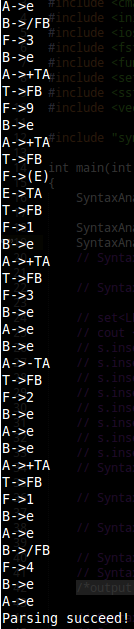
\includegraphics[width=\textwidth]{ll1yes.png}
                \caption{LL(1)解析成功}
                \label{fig:ll1yes}
        \end{subfigure}
        ~ %add desired spacing between images, e. g. ~, \quad, \qquad, \hfill etc.
          %(or a blank line to force the subfigure onto a new line)
        \begin{subfigure}[b]{0.25\textwidth}
                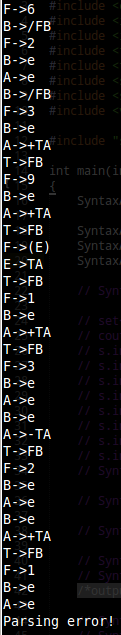
\includegraphics[width=\textwidth]{ll1no.png}
                \caption{LL(1)解析失败}
                \label{fig:ll1no}
        \end{subfigure}
        \caption{LL(1)语法分析器运行结果截图}\label{fig:ll1screenshot}
\end{figure}

\begin{figure}
        \centering        
        \begin{subfigure}[b]{0.4\textwidth}
                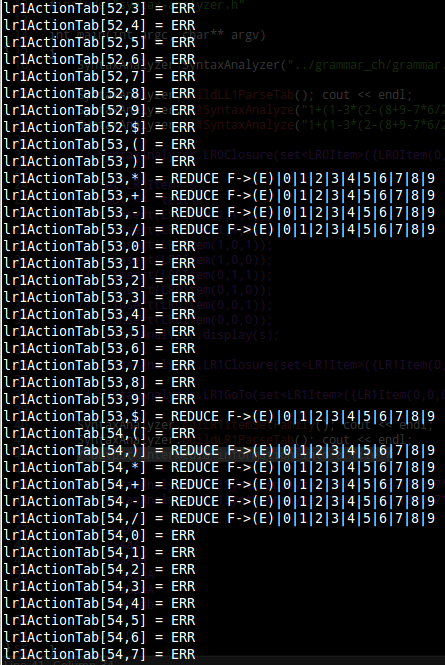
\includegraphics[width=\textwidth]{lr1actiontab.png}
                \caption{LR(1)Action分析表}
                \label{fig:ll1yes}
        \end{subfigure}
        \begin{subfigure}[b]{0.25\textwidth}
                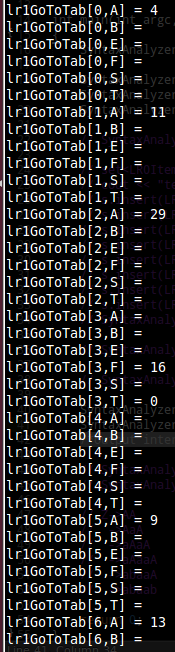
\includegraphics[width=\textwidth]{lr1gototab.png}
                \caption{LR(1)Goto分析表}
                \label{fig:ll1no}
        \end{subfigure}             
        \begin{subfigure}[b]{0.25\textwidth}
                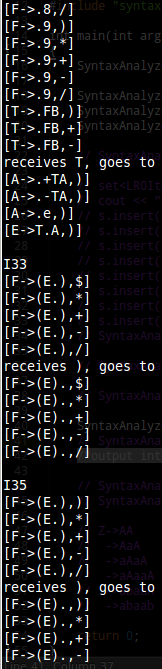
\includegraphics[width=\textwidth]{lr1itemsetfamily.png}
                \caption{LR(1)项集族}
                \label{fig:ll1}
        \end{subfigure}                  
        \caption{LR(1)语法分析器运行结果截图1}\label{fig:lr1screenshot1}
\end{figure}

\begin{figure}
        \centering        
        \begin{subfigure}[b]{0.5\textwidth}
                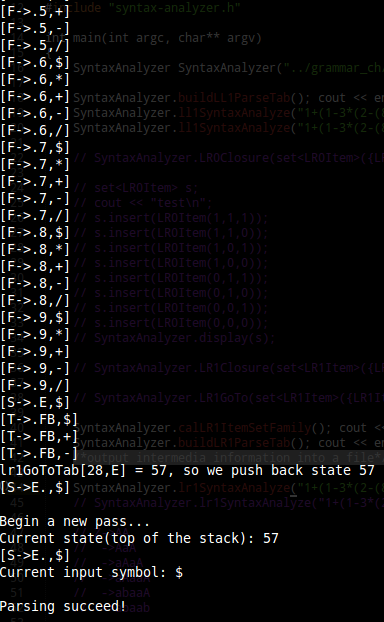
\includegraphics[width=\textwidth]{lr1yes.png}
                \caption{LR(1)解析成功}
                \label{fig:lr1yes}
        \end{subfigure}        
        \begin{subfigure}[b]{0.4\textwidth}
                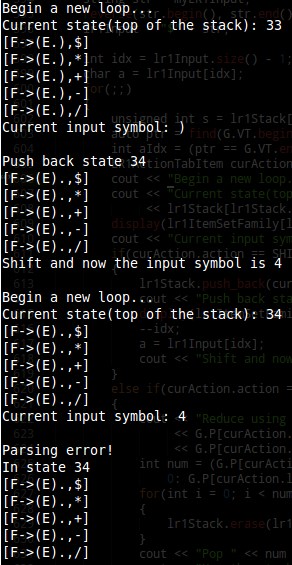
\includegraphics[width=\textwidth]{lr1no.png}
                \caption{LR(1)解析失败}
                \label{fig:lr1}
        \end{subfigure}             
        \caption{LR(1)语法分析器运行结果截图2}\label{fig:lr1screenshot2}
\end{figure}

\section{附录:文法的设计与实现} \label{sec: appendix}
\subsection{产生式数据结构的设计}
代码(代码清单~\ref{lst: productionrulelst})如下:
\begin{center}
\begin{lstlisting}[caption = {产生式数据结构的设计代码清单}, label = {lst: productionrulelst}]
class ProductionRule
{
public:
	ProductionRule();
	ProductionRule(const char& l, const vector<string>& r);

	void display();

	char lPart;
	vector<string> rPartSet;

private:

};

ProductionRule::ProductionRule()
{

}

ProductionRule::ProductionRule(const char& l, const vector<string>& r): lPart(l), rPartSet(r)
{

}

void ProductionRule::display()
{
	cout << lPart << "->";
	for(size_t i = 0; i < rPartSet.size(); ++i)
	{
		cout << rPartSet[i];
		if(i != rPartSet.size() - 1)
		{
			cout << "|";
		}
	}
}
\end{lstlisting}
\end{center}

\subsection{文法类的设计}
代码(代码清单~\ref{lst: grammarlst})如下:
\begin{center}
\begin{lstlisting}[caption = {文法类的设计代码清单}, label = {lst: grammarlst}]
class Grammar
{
public:
	Grammar(const string& filePath);

	void calNullableFirstFollow();

	void display();
	bool isNonTerminal(char ch);
	int getProductionRuleByLeft(ProductionRule& pr, char lPart); // return index of production rule which has lPart as left part
	set<char> getFirst(char ch);
	set<char> getFirst(string str);
	set<char> getFollow(char ch);

	vector<char> VN;
	vector<char> VT;
	vector<ProductionRule> P;
	char S;

	vector<bool> nullable; // for symbols in VN and VT, elements in VT are followed by elements in VN
	vector<set<char>> first; // for symbols in VN and VT, elements in VT are followed by elements in VN
	vector<set<char>> follow; // only for symbols in VN

private:
	
};
\end{lstlisting}
\end{center}

我们仅介绍构造函数~\texttt{calNullableFirstFollow} 成员函数的设计实现,其他函数仅用于输出信息和帮助对类的封装,不再赘述。

\subsubsection{构造函数的设计实现}
代码(代码清单~\ref{lst: constructlst})如下:
\begin{center}
\begin{lstlisting}[caption = {构造函数的设计实现代码清单}, label = {lst: constructlst}]
Grammar::Grammar(const string& filePath)
{
	ifstream f(filePath);
	assert(f);

	// file format
	// VNSize VN
	// VTSize VT
	// PSize
	// P
	// S

	int VNSize;
	f >> VNSize;
	VN.resize(VNSize);
	for(int i = 0; i < VNSize; ++i)
	{
		f >> VN[i];
	}

	int VTSize;
	f >> VTSize;
	VT.resize(VTSize);
	for(int i = 0; i < VTSize; ++i)
	{
		f >> VT[i];
	}

	struct functor: public binary_function<ProductionRule, char, bool>{
	public:
		bool operator ()(const ProductionRule pr, const char ch) const {
			return (pr.lPart == ch);
		}
	};

	int PSize;
	f >> PSize;
	string str;
	for(int i = 0; i < PSize; ++i)
	{
		f >> str;
		vector<string> v_pr = split(str, '>');
		v_pr[0].erase(v_pr[0].end() - 1);
		vector<string> v_pr_r = split(v_pr[1], '|');

		functor myFunctor;
		auto itr = find_if(P.begin(), P.end(), bind2nd(myFunctor, *(v_pr[0].begin())));
		if(itr == P.end())
		{
			ProductionRule pr;
			pr.lPart = *(v_pr[0].begin());
			for(size_t j = 0; j < v_pr_r.size(); ++j)
			{
				pr.rPartSet.push_back(v_pr_r[j]);
			}
			P.push_back(pr);
		}
		else
		{
			for(size_t j = 0; j < v_pr_r.size(); ++j)
			{
				P[itr - P.begin()].rPartSet.push_back(v_pr_r[j]);
			}
		}

	}

	f >> S;

	f.close();

	sort(VN.begin(), VN.end());
	sort(VT.begin(), VT.end());
	for(size_t i = 0; i < P.size(); ++i)
	{
		sort(P[i].rPartSet.begin(), P[i].rPartSet.end());
	}
	sort(P.begin(), P.end(),
		[](ProductionRule pr1, ProductionRule pr2)
		{
			return pr1.lPart < pr2.lPart?
				true: (pr1.lPart > pr2.lPart?
					false: pr1.rPartSet[0] < pr2.rPartSet[0]);
		});

	nullable.assign(VN.size(), false);
	first.assign(VN.size() + VT.size(), set<char>());
	follow.assign(VN.size(), set<char>());

	display();

	calNullableFirstFollow();
}
\end{lstlisting}
\end{center}

该文法类从格式化文本中读入信息并解析后完成初始化。

\subsubsection{\texttt{calNullableFirstFollow} 成员函数的设计实现}
代码(代码清单~\ref{lst: callst})如下:
\begin{center}
\begin{lstlisting}[caption = {\texttt{calNullableFirstFollow} 成员函数代码清单}, label = {lst: callst}]
void Grammar::calNullableFirstFollow()
{
	// calculate nullable

	for(size_t i = 0; i < P.size(); ++i)
	{
		for(size_t j = 0; j < P[i].rPartSet.size(); ++j)
		{
			if(P[i].rPartSet[j].size() == 1 && *(P[i].rPartSet[j].begin()) == 'e')
			{
				nullable[i] = true;
				break;
			}
		}
	}

	bool updated = true;
	while(updated)
	{
		updated = false;

		for(size_t i = 0; i < P.size(); ++i)
		{
			for(size_t j = 0; j < P[i].rPartSet.size(); ++j)
			{
				bool allNullable = true;
				for(size_t k = 0; k < P[i].rPartSet[j].size(); ++k)
				{
					auto ptr = find(VN.begin(), VN.end(), P[i].rPartSet[j][k]);
					if(ptr == VN.end() || !nullable[ptr - VN.begin()])
					{
						allNullable = false;
						break;
					}
				}

				if(allNullable && !nullable[i])
				{
					updated = true;
					nullable[i] = true;
					break;
				}
			}
		}
	}

	// calculate first

	for(size_t i = 0; i < VT.size(); ++i)
	{
		first[i].insert(VT[i]);
	}

	updated = true;
	while(updated)
	{
		updated = false;

		for(size_t i = 0; i < P.size(); ++i)
		{
			for(size_t j = 0; j < P[i].rPartSet.size(); ++j)
			{
				int idx = find(VN.begin(), VN.end(), P[i].lPart) - VN.begin() + VT.size();

				int l = 0;
				for(size_t k = 0; k < P[i].rPartSet[j].size(); ++k)
				{
					auto ptr = find(VN.begin(), VN.end(), P[i].rPartSet[j][k]);
					if(ptr == VN.end() || !nullable[ptr - VN.begin()])
					{
						break;
					}
					else
					{
						++l;

						int oldSize = first[idx].size();
						int newSize = 0;
						auto ptr = find(VN.begin(), VN.end(), P[i].rPartSet[j][k]);
						setUnion(first[idx], first[ptr - VN.begin() + VT.size()]);
						newSize = first[idx].size();
						if(oldSize != newSize)
						{
							updated = true;
						}
					}
				}

				/////////////////////////////////
				// cout << P[i].lPart << "->" << P[i].rPartSet[j] << " " << l << endl;

				int oldSize = first[idx].size();
				int newSize = 0;
				if(l >= P[i].rPartSet[j].size())
				{
					first[idx].insert('e');
					newSize = first[idx].size();
				}
				else
				{
					auto ptr = find(VN.begin(), VN.end(), P[i].rPartSet[j][l]);
					if(ptr == VN.end())
					{
						if(P[i].rPartSet[j][l] != 'e')
						{
							setUnion(first[idx], first[find(VT.begin(), VT.end(), P[i].rPartSet[j][l]) - VT.begin()]);

							/////////////////////////////////
							// cout << i << " " << idx << " ";
							// ::display(first[find(VT.begin(), VT.end(), P[i].rPartSet[j][l]) - VT.begin()]); cout << endl << endl;
						}
						else
						{
							setUnion(first[idx], set<char>({'e'}));
						}
					}
					else
					{
						setUnion(first[idx], first[ptr - VN.begin() + VT.size()]);
					}

					newSize = first[idx].size();
				}
			
				if(oldSize != newSize)
				{
					updated = true;
				}
			}
		}
	}

	// sth about $ and e

	follow[find(VN.begin(), VN.end(), S) - VN.begin()].insert('$');

	updated = true;
	while(updated)
	{
		updated = false;

		for(size_t i = 0; i < P.size(); ++i)
		{
			for(size_t j = 0; j < P[i].rPartSet.size(); ++j)
			{
				int idx = find(VN.begin(), VN.end(), P[i].lPart) - VN.begin();

				for(size_t k = 0; k < P[i].rPartSet[j].size(); ++k)
				{
					bool allNullable1 = true;
					for(size_t cnt = k + 1; cnt < P[i].rPartSet[j].size(); ++cnt)
					{
						if(P[i].rPartSet[j][cnt] != 'e')
						{
							auto cntPtr = find(VN.begin(), VN.end(), P[i].rPartSet[j][cnt]);
							if(cntPtr == VN.end() || !nullable[cntPtr - VN.begin()])
							{
								allNullable1 = false;
								break;
							}
						}
						else
						{
							break;
						}
					}
					if(allNullable1)
					{
						auto kPtr = find(VN.begin(), VN.end(), P[i].rPartSet[j][k]);
						if(kPtr != VN.end())
						{
							int oldSize = follow[kPtr - VN.begin()].size();
							setUnion(follow[kPtr - VN.begin()], follow[idx]);
							int newSize = follow[kPtr - VN.begin()].size();
							if(oldSize != newSize)
							{
								updated = true;
							}
						}
					}

					for(size_t l = k + 1; l < P[i].rPartSet[j].size(); ++l)
					{
						bool allNullable2 = true;
						for(int cnt = k + 1; cnt < l - 1; ++cnt)
						{
							if(P[i].rPartSet[j][cnt] != 'e')
							{
								auto cntPtr = find(VN.begin(), VN.end(), P[i].rPartSet[j][cnt]);
								if(cntPtr == VN.end() || !nullable[cntPtr - VN.begin()])
								{
									allNullable2 = false;
									break;
								}
							}
							else
							{
								break;
							}
						}
						if(allNullable2)
						{
							auto kPtr = find(VN.begin(), VN.end(), P[i].rPartSet[j][k]);
							if(kPtr != VN.end())
							{
								auto lPtr = find(VN.begin(), VN.end(), P[i].rPartSet[j][l]);
								int lIdx = (lPtr == VN.end())?
									(find(VT.begin(), VT.end(), P[i].rPartSet[j][l]) - VT.begin()):
									(lPtr - VN.begin() + VT.size());
								int oldSize = follow[kPtr - VN.begin()].size();
								set<char> __first__ = first[lIdx];
								__first__.erase('e');
								setUnion(follow[kPtr - VN.begin()], __first__);
								int newSize = follow[kPtr - VN.begin()].size();
								if(oldSize != newSize)
								{
									updated = true;
								}
							}
						}
					}
				}
			}
		}
	}

	// display nullable
	cout << "nullable" << endl;
	for(size_t i = 0; i < nullable.size(); ++i)
	{
		cout << VN[i] << ": " << ((nullable[i])? "nullable": "not nullable") << endl;
	}
	cout << endl;

	// display first
	cout << "first" << endl;
	for(size_t i = 0; i < first.size(); ++i)
	{
		if(i < VT.size())
		{
			cout << VT[i] << ": ";
			::display(first[i]);
			cout << endl;
		}
		else
		{
			cout << VN[i - VT.size()] << ": ";
			::display(first[i]);
			cout << endl;
		}
	}
	cout << endl;

	// display follow
	cout << "follow" << endl;
	for(size_t i = 0; i < follow.size(); ++i)
	{
		cout << VN[i] << ": ";
		::display(follow[i]);
		cout << endl;
	}
	cout << endl;
}
\end{lstlisting}
\end{center}

递归的计算方法要求指定求值顺序这一问题,为了避开这一棘手的问题,我们使用迭代至不懂点的方法求~\texttt{nullable} 集,\texttt{first} 集和~\texttt{follow}集。需要说明的是,我们使用字符~\texttt{e} 表示空串,并对它进行不同于其他终结符的特殊处理。

\end{CJK*}
\end{document}
